\documentclass[aspectratio=169,11pt]{beamer}
% Shared preamble for the CogLean decks.
% Build the slides alone, or with speaker notes (see the Makefile):
%   pdflatex deck.tex                                   -> slides
%   pdflatex -jobname=deck-notes "\def\withnotes{}\input{deck.tex}"  -> slides + notes
\usetheme{default}
\usecolortheme{seahorse}
\setbeamertemplate{navigation symbols}{}
\setbeamertemplate{footline}[frame number]
\setbeamerfont{note page}{size=\small}
\ifdefined\withnotes
  \setbeameroption{show notes}
\fi
\usepackage[T1]{fontenc}
\usepackage{lmodern}
\usepackage{booktabs}
\usepackage{amsmath,amssymb}
\usepackage{tikz}
\usetikzlibrary{positioning,arrows.meta,shapes.misc}
\tikzset{
  box/.style={draw, rounded corners, align=center, minimum height=8mm, inner sep=4pt, fill=blue!6},
  arr/.style={-{Stealth[length=2mm]}, thick}
}
\newcommand{\code}[1]{\texttt{#1}}
\newcommand{\has}{\textbf{has}}
\newcommand{\lacks}{\textcolor{red!70!black}{lacks}}
\newcommand{\never}{\textcolor{red!70!black}{\textbf{never}}}
\newcommand{\canhold}{can hold}


\title{Recognition, retrieval and confident errors}
\subtitle{Multi-digit addition, a blind simulation, swapping memories, and a second task}
\author{Jeff Shrager}
\date{October 2026}

\begin{document}

\begin{frame}
  \titlepage
\end{frame}
\note{
This talk follows one model from its postulates to a theorem that two different tasks inherit. It's a model of multi-digit addition that combines two classic theories, EPAM and the distributions-of-associations model. I'll state its central prediction, confident errors, show a worked case, describe how we checked the formalization with a blind simulation, swap EPAM's memory for ACT-R's, extract the general composition, apply it to naming people, and derive the result from laws. Everything I quote is a theorem or an exact computation checked by Lean.
}

\begin{frame}{Two theories, combined}
  \begin{columns}[T]
    \column{0.5\textwidth}
    \textbf{EPAM} (Feigenbaum 1959)
    \begin{itemize}\small
      \item Stimuli are feature codes.
      \item A discrimination net sorts a code by testing features, down to a stored image.
      \item Learning grows a test only where two codes are confused, on the first difference noticed.
      \item So an unfamiliar code that agrees on every tested feature is \emph{recognized as} a familiar one.
    \end{itemize}
    \column{0.5\textwidth}
    \textbf{Distributions of associations} (Siegler \& Shrager 1984)
    \begin{itemize}\small
      \item Each problem has associations to answers, with strengths.
      \item Sample an answer in proportion to strength; state it if it clears a confidence criterion; try up to $n$ times.
      \item Otherwise, use a backup strategy.
      \item Retrieval is used with probability $1-(1-R)^n$.
    \end{itemize}
  \end{columns}
\end{frame}
\note{
Here are two classic theories. EPAM, Feigenbaum's model of verbal learning: stimuli are feature codes, sorted through a discrimination net of feature tests, and the net grows a new test only where two codes get confused. So an unfamiliar code that matches a familiar one on every tested feature gets recognized as that familiar one. And the distributions-of-associations model of strategy choice, which Bob Siegler and I proposed: each problem has associations to answers; you sample an answer in proportion to its strength, state it if it clears a confidence criterion, try a few times, and otherwise fall back on a backup strategy such as counting.
}

\begin{frame}{The multi-digit model}
  \begin{center}
  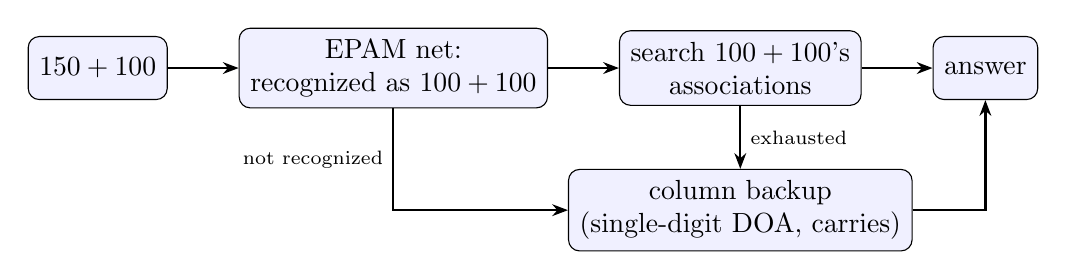
\begin{tikzpicture}[node distance=9mm]
    \node[box] (p) {$150+100$};
    \node[box, right=of p] (r) {EPAM net:\\recognized as $100+100$};
    \node[box, right=of r] (s) {search $100+100$'s\\associations};
    \node[box, below=8mm of s] (b) {column backup\\(single-digit DOA, carries)};
    \node[box, right=of s] (a) {answer};
    \draw[arr] (p) -- (r); \draw[arr] (r) -- (s); \draw[arr] (s) -- (a);
    \draw[arr] (r) |- node[pos=0.25, left]{\scriptsize not recognized} (b);
    \draw[arr] (s) -- node[right]{\scriptsize exhausted} (b);
    \draw[arr] (b) -| (a);
  \end{tikzpicture}
  \end{center}
  \begin{itemize}\small
    \item Every postulate is a parameter: the encoding, the net, the strengths, the criterion, the search length, the backup.
    \item 18 predictions, each proved for every choice of them.
  \end{itemize}
\end{frame}
\note{
Combine them and you get a model of three-digit addition. A problem like 150 plus 100 is first recognized by an EPAM net, perhaps as the familiar 100 plus 100. Then retrieval searches the recognized problem's associations. If nothing is recognized, or retrieval comes up empty, the child works it out column by column, where each column is itself a single-digit trial of retrieval or backup, with carries. Every postulate here is a parameter: the encoding, the net, the strengths, the criterion, the search length, the backup. The model yields eighteen predictions, each proved for every choice of those parameters.
}

\begin{frame}{Confident errors}
  Let a familiar problem $q$ have \emph{sharp} associations (only its correct sum clears the criterion), and let $x$, with a different sum, be recognized as $q$. Then:
  \begin{enumerate}
    \item on $q$, whole-problem retrieval never errs;
    \item on $x$, every whole-problem answer is wrong;
    \item $x$ uses the backup exactly as rarely as $q$ does: $(1-R_q)^n$.
  \end{enumerate}
  \bigskip
  In DOA alone, errors and backup use rise together. Confusion breaks the tie: a retrieved, wrong answer with no extra backup use.
\end{frame}
\note{
Here is the prediction neither theory makes alone. Suppose a familiar problem q has sharp associations, meaning only its correct sum clears the criterion, and a stranger x with a different sum is recognized as q. Then q is never answered wrongly by retrieval; every retrieved answer to x is wrong; and x falls back on the columns exactly as rarely as q does. In the associations model alone, errors and backup use rise and fall together. Confusion breaks that tie: you get a retrieved, wrong answer with no extra backup use. Notice that I don't say fast: the model has no timing, so that would need more.
}

\begin{frame}{A worked case}
  \begin{itemize}
    \item Encoding: each digit in four bits (24 features). The net learns $100+100$ and $100+200$, which differ only in the second addend's hundreds digit, so that is all it tests.
    \item Associations: $.90$ on each problem's sum, $.01$ elsewhere; criterion $.50$; search length 1.
    \item $150+100$ is recognized as $100+100$.
  \end{itemize}
  \bigskip
  \begin{center}
  \begin{tabular}{lc}
    \toprule
    $150+100$ answered $200$, by retrieval & $45/46$\\
    $150+100$ sent to the columns & $1/46$\\
    \bottomrule
  \end{tabular}
  \end{center}
\end{frame}
\note{
To see it concretely: encode each digit in four bits. A net that has learned 100 plus 100 and 100 plus 200 only needs to test the second addend's hundreds digit to tell them apart. So 150 plus 100 slips through as 100 plus 100. With these strengths and a single search, it's answered 200 by retrieval with probability 45 over 46, and sent to the columns with probability 1 over 46. With the column problem solver doing the columns from single-digit facts, it's then right about two thirds of the time, so correct overall only about one and a half percent of the time. These numbers are just an illustration, computed exactly; the structure, confident errors, holds for every choice of parameters.
}

\begin{frame}{Checking the formalization: a blind simulation}
  The proofs show the predictions follow from the Lean definitions, not that the definitions say what the prose model says.
  \medskip
  \begin{enumerate}\small
    \item A prose specification, with no Lean names or predictions.
    \item Predictions \textbf{preregistered} and committed before the simulator existed.
    \item A fresh AI agent, given only the prose, wrote a Python simulator. Its tool use was audited.
    \item A harness compared it with the preregistered predictions and with Lean's exact distributions.
  \end{enumerate}
  \medskip
  \textbf{Result}: no failures. 243 outcome frequencies on 4 instances matched Lean's exact values, and every applicable prediction passed.
\end{frame}
\note{
The proofs show that the predictions follow from the Lean definitions, not that the definitions say what the prose model says. So we checked that link with a blind simulation. We wrote a prose specification with no Lean in it, and preregistered the predictions before any simulator existed. A fresh AI agent, given only the prose, wrote a Python simulator, and a harness compared it with the predictions and with Lean's exact distributions. There were no failures: 243 outcome frequencies matched Lean's exact values. It also found five vacuous predictions, a gap in the formalization, and a prediction that depends on a choice the model leaves open. There's a separate talk on this.
}

\begin{frame}{Memory as a parameter}
  The recognition step is now an interface: memory takes a probe and returns a \emph{distribution} over stored items (or nothing).
  \medskip
  \begin{itemize}\small
    \item EPAM's net is one memory: deterministic.
    \item ACT-R's declarative memory is another: base-level activation that decays, partial matching, a retrieval threshold.
    \item With decay 1 and temperature 1, ACT-R's retrieval probabilities are exactly rational, so Lean computes them exactly.
  \end{itemize}
  \medskip
  Each prediction now states the law of memory it needs. Swap the memory and keep every theorem whose laws still hold.
\end{frame}
\note{
Next we made memory a parameter. The recognition step is now an interface: memory takes a probe and returns a probability distribution over stored items, or nothing. EPAM's net is one memory, and it's deterministic. ACT-R's declarative memory is another, with base-level activation that decays, partial matching and a retrieval threshold. With decay one and temperature one, ACT-R's retrieval probabilities are exactly rational, so Lean can compute them exactly. Each prediction now states the law of memory it needs, so when we swap memories we keep every theorem whose laws still hold.
}

\begin{frame}{The same problems, two memories}
  \small
  \begin{center}
  \begin{tabular}{lcc}
    \toprule
    & EPAM & ACT-R\\
    \midrule
    $150+100$ answered $200$ (the neighbour's sum) & $45/46$ & $225/529$\\
    $150+100$ answered $300$ (differs on a tested digit) & $0$ & $225/1058$\\
    $150+100$ sent to the columns & $1/46$ & $383/1058$\\
    errors on the practiced $100+100$ & $0$ & $225/782$\\
    the same, after also studying $100+300$ & $0$ & $3375/5842$\\
    \bottomrule
  \end{tabular}
  \end{center}
  \normalsize
  ACT-R: confusion is graded, nothing is retrieved for certain, and new practice interferes with old.
\end{frame}
\note{
Here are the same problems run through both memories. With EPAM, 150 plus 100 is answered 200 with probability 45 over 46, and never 300; a practiced problem never errs, and learning something new doesn't change that. With ACT-R, the confusion is graded: 150 plus 100 can be taken for either familiar problem, even the practiced 100 plus 100 sometimes errs, and studying 100 plus 300 more than doubles its errors. EPAM's zeros are theorems. ACT-R's departures are proved on this instance and explained by laws it lacks.
}

\begin{frame}{The composition, extracted}
  The model's trial is one case of a general composition, now in the shared library:
  \medskip
  \begin{center}
  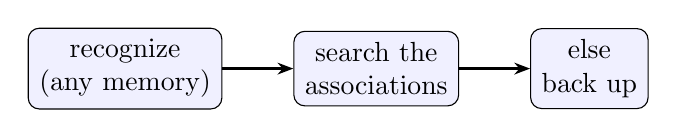
\begin{tikzpicture}[node distance=9mm]
    \node[box] (r) {recognize\\(any memory)};
    \node[box, right=of r] (s) {search the\\associations};
    \node[box, right=of s] (b) {else\\back up};
    \draw[arr] (r) -- (s); \draw[arr] (s) -- (b);
  \end{tikzpicture}
  \end{center}
  \begin{itemize}\small
    \item Over any problems and any answers, with ``the correct answer'' a parameter.
    \item Confident errors, and the rest, are proved once for the composition.
    \item Multi-digit addition is an instance: one bridge lemma carries every probability across, and its theorems keep their names.
  \end{itemize}
\end{frame}
\note{
The model's trial turns out to be one case of a general composition: recognize with any memory, search the recognized item's associations, else back up. We moved that into the shared library, over any problems and any answers, with the correct answer as a parameter, and proved confident errors there, once. Multi-digit addition is now just an instance: one bridge lemma carries every probability across, and all its theorems keep their names. Its definitions were left untouched, so the numbers exported for the simulation and the paper are byte-identical.
}

\begin{frame}{A second task: naming people}
  Faces are codes; familiar Ann (000) and Bob (110); stranger Carl (100), one feature from each. The backup is ``don't know''.
  \medskip
  \small
  \begin{center}
  \begin{tabular}{lcc}
    \toprule
    & EPAM & ACT-R\\
    \midrule
    Carl named Bob & $45/46$ & $225/391$\\
    Carl named Ann & $0$ & $225/782$\\
    Carl: ``don't know'' & $1/46$ & $107/782$\\
    Bob: ``don't know'' & $1/46$ & $229/2254$\\
    Bob named Ann & $0$ & $225/2254$\\
    \bottomrule
  \end{tabular}
  \end{center}
  \medskip
  \normalsize
  With EPAM, \emph{confident misnaming} is inherited from the composition's theorem, for every search length. No arithmetic anywhere.
\end{frame}
\note{
To show it isn't about arithmetic, here is a second task through the same composition: naming people. Faces are codes; Ann and Bob are familiar; Carl is a stranger who resembles both. With EPAM's memory, the confident-errors theorem is simply inherited: Carl is confidently misnamed Bob, and he says don't know exactly as rarely as Bob himself does. With ACT-R's memory, the misnaming is graded: Carl can be taken for either familiar person, and he says don't know more often than Bob.
}

\begin{frame}{From laws: which memories give confident errors?}
  \textbf{Theorem.} Any memory with three laws (\emph{determinacy}, \emph{certainty}, \emph{stability}) produces confident errors whenever a stranger can be taken for a studied item with sharp associations.
  \bigskip
  \begin{itemize}
    \item In the matrix of memory families, only discrimination (EPAM) has all three.
    \item Face naming's confident misnaming is derived this way, from EPAM's matrix cells plus one computed fact (Carl can be taken for Bob).
    \item The evidence judges that people lack certainty. So explaining confident errors in people needs a graded version: these laws with high probability, not probability 1.
  \end{itemize}
\end{frame}
\note{
Here's where the two halves meet. Confident errors can be derived from three laws: any memory with determinacy, certainty and stability produces them, whenever a stranger can be taken for a studied item. So the matrix answers the question of which memory families produce confident errors: only discrimination. And since the evidence suggests people lack certainty, explaining confident errors in people will need a graded version of this theorem.
}

\begin{frame}{Limits, and next}
  \begin{itemize}
    \item \textbf{No timing.} ``Retrieved, with no extra backup use'' is what is proved; ``fast'' needs a timing model.
    \item \textbf{One trial at a time.} Learning across trials (feedback, discrimination, strengthening) makes memory states random; the predicted sequence (confident error, then column work, then fluent retrieval) is the next target.
    \item \textbf{Formal fidelity.} ACT-R here is one restricted formalization; checking it against PyACTUp, the community implementation, is planned.
    \item \textbf{A graded confident-errors theorem}, for memories without certainty.
  \end{itemize}
\end{frame}
\note{
Some limits. The model has no timing, so what is proved is a retrieved answer with no extra backup use, not a fast one. It treats one trial at a time: learning across trials, where feedback discriminates and strengthens, makes memory states random, and the predicted sequence of a confident error, then column work, then fluent retrieval is the next target. Our ACT-R is one restricted formalization, which we plan to check against PyACTUp. And we need a graded version of the confident-errors theorem, for memories that are never certain.
}

\end{document}
